% soutenance_schemas.tex
% =====================================================================
% Schemas TikZ de `soutenance_20min.tex` : la carte des idees et le schema
% de l'identite de course.
%
% Fichier separe pour la meme raison que `point_encadrant_schemas.tex` :
% `verif_chiffres_tex.py` ramasserait les coordonnees TikZ comme des mesures.
% AUCUN chiffre de mesure ici ; les schemas sont stylises, sans donnees.
% =====================================================================

\usetikzlibrary{positioning, arrows.meta, calc}

\definecolor{mTheorie}{RGB}{31,58,104}
\definecolor{mDate}{RGB}{138,28,28}
\definecolor{mPreuve}{RGB}{38,92,58}
\definecolor{mEteint}{gray}{0.74}

% ---------------------------------------------------------------------
% \carte[hauteur]{k} : la carte des idees.
%   k = 0 : tout est actif (ouverture et conclusion)
%   k = 1, 2, 3 : seule la partie k est en couleur, le reste est grise
%   hauteur : fraction de \textheight (0.80 par defaut)
% Les fleches en pointille relient les parties ; elles sont commentees a
% l'oral plutot qu'etiquetees, faute de place entre les colonnes.
% ---------------------------------------------------------------------
\newcommand{\carte}[2][0.80]{%
  \colorlet{cUn}{mEteint}\colorlet{cDeux}{mEteint}\colorlet{cTrois}{mEteint}%
  \colorlet{tUn}{mEteint}\colorlet{tDeux}{mEteint}\colorlet{tTrois}{mEteint}%
  \ifnum#2=0 \colorlet{cUn}{mTheorie}\colorlet{cDeux}{mDate}\colorlet{cTrois}{mPreuve}%
    \colorlet{tUn}{black}\colorlet{tDeux}{black}\colorlet{tTrois}{black}\fi
  \ifnum#2=1 \colorlet{cUn}{mTheorie}\colorlet{tUn}{black}\fi
  \ifnum#2=2 \colorlet{cDeux}{mDate}\colorlet{tDeux}{black}\fi
  \ifnum#2=3 \colorlet{cTrois}{mPreuve}\colorlet{tTrois}{black}\fi
  \resizebox{!}{#1\textheight}{%
  \begin{tikzpicture}[
      font=\normalsize, align=center,
      boite/.style={draw, line width=1pt, rounded corners=3pt, inner sep=4pt,
                    text width=4.3cm, minimum height=1.05cm},
      un/.style={boite, draw=cUn, text=tUn},
      deux/.style={boite, draw=cDeux, text=tDeux},
      trois/.style={boite, draw=cTrois, text=tTrois},
      tete/.style={font=\bfseries\normalsize, text width=4.8cm},
      fl/.style={-{Stealth[length=2.4mm]}, line width=0.9pt},
      lien/.style={-{Stealth[length=2.4mm]}, line width=0.9pt, dashed},
    ]
    \node[boite, draw=black, fill=black!4, text width=12cm, minimum height=0.8cm] (P) at (5.6,0.15)
      {\textbf{The paper:} the stronger the drift, the faster the repair, the fewer the alarms};

    \node[tete, text=cUn]    (H1) at (0,-1.05)    {I.\ The race, formally};
    \node[tete, text=cDeux]  (H2) at (5.6,-1.05)  {II.\ The repair date};
    \node[tete, text=cTrois] (H3) at (11.2,-1.05) {III.\ Evidence vs threshold};
    \draw[fl, black!55] (P.south) -- ++(0,-0.25) -| (H1.north);
    \draw[fl, black!55] (P.south) -- (H2.north);
    \draw[fl, black!55] (P.south) -- ++(0,-0.25) -| (H3.north);

    \node[un] (A1) at (0,-2.1)  {The miss is well defined, its probability identified};
    \node[un] (A2) at (0,-3.45) {The blind spot holds whatever the dependence};
    \node[un] (B1) at (0,-4.8)  {Independent trees overstate the speed of repair};

    \node[deux] (C1) at (5.6,-2.1)  {The first replacement is the earliest date};
    \node[deux] (E1) at (5.6,-3.45) {It fires as fast when nothing changes};
    \node[deux] (D1) at (5.6,-4.8)  {When it fires, half the evidence is there};
    \node[deux] (D2) at (5.6,-6.15) {Indicators form two groups, weakly linked};

    \node[trois] (C2) at (11.2,-2.1)  {The alarm is a function of the error path};
    \node[trois] (K)  at (11.2,-3.45) {Detector first \emph{iff} it reaches $\lambda$ before the repair};
    \node[trois] (S)  at (11.2,-4.8)  {That evidence sets the transition and the paradox};
    \node[trois] (T)  at (11.2,-6.15) {Detecting is not winning};

    \node[boite, draw=black!55, text=black!80, dashed, text width=7cm, minimum height=0.8cm] (O) at (5.6,-7.45)
      {\textbf{Open:} a reference for adaptation itself};

    \draw[fl, cUn]    (A1) -- (A2);
    \draw[fl, cDeux]  (C1) -- (E1);
    \draw[fl, cDeux]  (E1) -- (D1);
    \draw[fl, cDeux]  (D1) -- (D2);
    \draw[fl, cTrois] (C2) -- (K);
    \draw[fl, cTrois] (K) -- (S);
    \draw[fl, cTrois] (S) -- (T);
    \draw[lien, black!55] (B1.east) -- (D1.west);
    \draw[lien, black!55] (D1.east) -- (S.west);
    \draw[lien, black!55] (D2.south) -- (O.north);
  \end{tikzpicture}}%
}

% ---------------------------------------------------------------------
% \schemaidentite : la pile S_t, le premier remplacement, deux seuils.
% Stylise, sans donnees.
% ---------------------------------------------------------------------
\newcommand{\schemaidentite}{%
  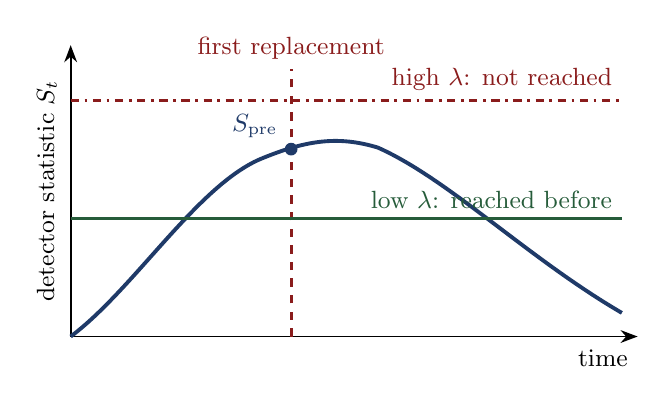
\begin{tikzpicture}[x=1cm, y=1cm, font=\small]
    \draw[-{Stealth}, line width=0.7pt] (0,0) -- (7.2,0);
    \node[below left] at (7.2,-0.05) {time};
    \draw[-{Stealth}, line width=0.7pt] (0,0) -- (0,3.7);
    \node[rotate=90, above] at (-0.05,1.85) {detector statistic $S_t$};
    \draw[line width=1.4pt, mTheorie]
      (0,0) .. controls (0.8,0.6) and (1.6,1.9) .. (2.4,2.25)
            .. controls (3.0,2.5) and (3.4,2.55) .. (3.9,2.4)
            .. controls (4.8,2.0) and (5.8,1.0) .. (7.0,0.3);
    \draw[dashed, mDate, line width=1pt] (2.8,0) -- (2.8,3.4);
    \node[above, text=mDate] at (2.8,3.4) {first replacement};
    \fill[mTheorie] (2.8,2.38) circle (2.3pt);
    \node[above left, text=mTheorie] at (2.75,2.4) {$S_{\mathrm{pre}}$};
    \draw[mPreuve, line width=1pt] (0,1.5) -- (7.0,1.5);
    \node[above left, text=mPreuve] at (7.0,1.5) {low $\lambda$: reached before};
    \draw[mDate, line width=1pt, dash dot] (0,3.0) -- (7.0,3.0);
    \node[above left, text=mDate] at (7.0,3.0) {high $\lambda$: not reached};
  \end{tikzpicture}%
}
